\chapter{Applicazione Mobile}\label{chap:mobile-app}

In questo capitolo verrà presentato un esempio di applicazione mobile in grado di connettersi al CS e di eseguire le operazione di prenotazione e ritiro delle ricariche. Scopo dell'applicazione è permettere all'utente di interagire con la smart-city per ridurre le problematiche derivanti dall'utilizzo di veicoli elettrici. La comunicazione avviene mediante i protocolli visti nella Sez. ~\ref{sec:protocol}.

Inizialmente era possibile eseguire solo operazioni di prenotazione e cancellazione di ricariche e il funzionamento era subordinato alla presenza del simulatore. Il funzionamento è stato ampliato con la possibilità di connettersi tramite Bluetooth a un veicolo reale, opportunità concessa dal \emph{Centro Ricerche Fiat} (CRF).

A questo ho aggiunto la possibilità di analizzare il profilo altimetrico che separa il dispositivo mobile da un determinato EVSE per consentire previsioni più accurate sui consumi necessari a raggiungerlo.

\section{Architettura}

La piattaforma scelta per lo sviluppo è Android, versione 4.0.3 o superiori, in quanto vantano maggiori performance e un interfaccia utente più gradevole e facile da programmare. La libreria di base per interfacciarsi con il SIB è quella esposta nella sezione \ref{subsec:ioe-lib}.

La comunicazione con il CS avviene tramite scambio di messaggi con il \emph{City SIB}, mentre le informazioni relative al veicolo, in particolar modo se quest'ultimo è simulato, giungono dal \emph{Dash SIB}. È possibile collegare l'applicazione ad un veicolo reale che sia provvisto della tecnologia Blue\&{}Me di Fiat. I dati del profilo altimetrico sono ottenuti tramite una libreria, UniboGeoTools (App. \ref{app:unibo-geo-tools}), che ho sviluppato appositamente per l'occasione.

\subsection{Android}

Malgrado Android sia ampiamente conosciuto penso sia necessario spendere qualche parola per introdurre i concetti che stanno alla base della programmazione di applicazioni basate su questo sistema operativo per una maggiore comprensione del resto della trattazione.

Android è un sistema operativo Linux-based, Open Source, orientato all'utilizzo su dispositivi mobili anche se negli ultimi anni sta prendendo sempre più piede all'interno di smart-tv, dispositivi embedded, mini computer ecc\dots

La programmazione di applicazioni avviene attraverso una versione ad-hoc del linguaggio Java che, seppur eseguita su una virtual machine diversa dalla JVM (Dalvik), ne mantiene quasi tutte le caratteristiche e la libreria di base. Naturalmente oltre alla libreria standard vengono fornite le API che permettono l'interfacciamento con le funzionalità di Android.

\subsubsection{Activity}

Le Activity sono uno degli elementi centrali della programmazione di applicazioni Android (\cite{html:android}). In genere un Activity rappresenta una singola schermata della nostra applicazione. Le applicazioni possono definire una o più Activity per trattare diverse fasi del software, e generalmente ognuna di esse corrisponde ad un azione specifica che può essere eseguita dall'utente. 

In un determinato istante ci può essere una sola Activity attiva. Mentre quelle non attive possono essere terminate in qualunque momento dal sistema operativo per recuperare memoria. Il programmatore deve quindi prevedere per ogni Activity il codice necessario a salvarne lo stato per consentirne il ripristino in caso di necessità. Come si può vedere in figura \ref{fig:android-activity} le Activity di Android hanno un ciclo di vita abbastanza complesso. 

\subsubsection{Service}

Un Service è un processo che gira in background (concetto molto simile al daemon in ambiente Unix) e può essere avviato e comandato da Activity o altri Service. La classe Service viene utilizzata per creare componenti software che possono svolgere attività in modo ``invisibile'', senza interfaccia utente.

Un Service può trovarsi in due stati(\cite{emanuele:android}):

\begin{itemize}
	\item \textbf{Started}: un servizio si trova in questo stato quando viene invocato il metodo startService() e gira in background per un tempo indefinito o finché il componente che lo ha invocato non viene distrutto (Fig. \ref{fig:android-service} sinistra).
	\item \textbf{Bounded}: un servizio si trova in questo stato quando si invoca il metodo bindService(). I servizi di questo tipo offrono un'interfaccia per la comunicazione client-server, affinché le componenti che invocano il servizio possono interagire con esso. In questo caso il servizio è attivo solo finché le componenti sono associate con esso (Fig. \ref{fig:android-service} destra).
\end{itemize}

\noindent
Un Servizio avviato ha una priorità più alta rispetto ad Activity in stato di inattività. Un Service ha quindi minore probabilità di essere terminato dal gestore delle risorse di Android. L'unica ragione per cui Android potrebbe fermare un Service prematuramente è per fornire risorse addizionali al componente software in primo piano (normalmente una Activity).

I servizi vengono avviati nel thread principale del processo. Ne consegue che se eseguissero operazioni bloccanti o ad alto consumo di risorse potrebbero portare al blocco dell'intero processo facendo generare ad Android un errore del tipo: ``Application Not Responding''. Per evitare questo è bene far gestire il servizio in un thread separato.

\begin{figure}[H]
        \centering
        \begin{subfigure}[b]{0.49\textwidth}
			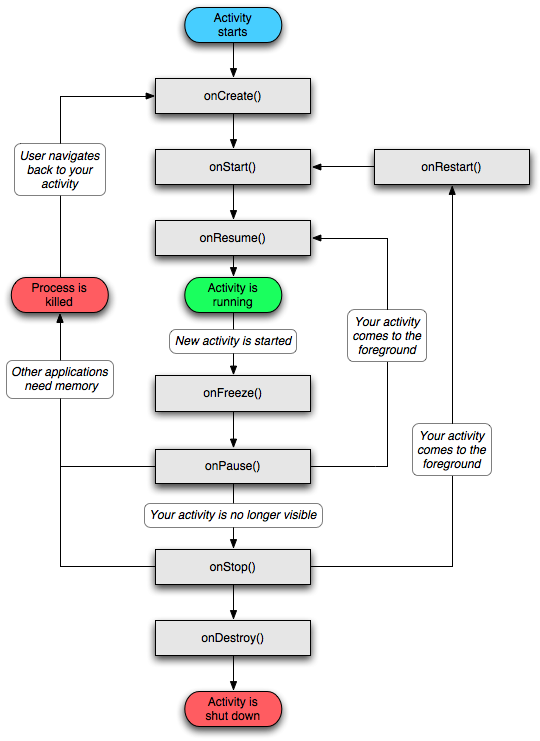
\includegraphics[width=\textwidth]{assets/android-activity.png}
			\caption{Ciclo di vita di un Activity Android}
			\label{fig:android-activity}
		\end{subfigure}
        \begin{subfigure}[b]{0.49\textwidth}
			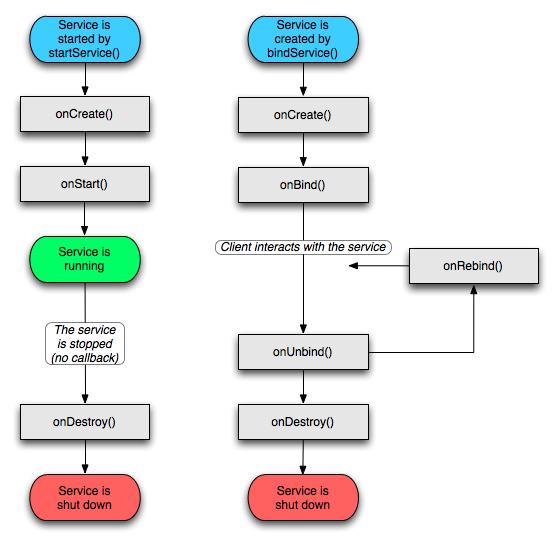
\includegraphics[width=\textwidth]{assets/android-service.png}
			\caption{Ciclo di vita di un Service Android}
			\label{fig:android-service}
		\end{subfigure}
        \caption{Ciclo di vita Activity e Service Android}
\end{figure}

\subsection{Blue\&{}Me}

Il Blue\&{}Me è il risultato di un accordo tra Fiat Auto e Microsoft con l'obiettivo di progettare sistemi telematici innovativi per l'automotive, presentato nel 2006 (\cite{al2012android}). Basato sulla piattaforma Windows Embedded Automotive (connubio del sistema operativo Windows CE con il middleware Microsoft Auto) è sviluppato da Magneti Marelli, azienda del gruppo FIAT, in collaborazione con Microsoft (\cite{wiki:blue-me}).

Blue\&{}Me è un sistema viva voce con tecnologia Bluetooth, riconoscimento vocale, lettore multimediale con presa USB e comandi al volante. Fiat Auto e Microsoft, con il supporto di Magneti Marelli, offrono una piattaforma adattabile alla maggior parte dei telefoni cellulari e lettori musicali. Il sistema si interfaccia con il cellulare mediante la tecnologia Bluetooth e permette al guidatore di rispondere al telefono senza tenerlo in mano. 

La funzionalità del Blue\&{}Me più appetibile per i nostri scopi è il monitoraggio dei parametri del veicolo. Nel progetto ho lavorato con un prototipo di Fiat Daily elettrico opportunamente modificato per trasmettere i dati della batteria tramite tecnologia Bluetooth. La connessione è stata possibile grazie alle librerie rese disponibili dal CRF unitamente ad un efficace esempio applicativo. Fiat è infatti uno dei partner del progetto IoE.

L'interazione con il Blue\&{}Me è di tipo push: ogniqualvolta la centralina della macchina rileva che un dato è variato (in base ad una determinata soglia) allora ``scrive'' invia tramite interfaccia Bluetooth. Questo implica dall'altro lato dell'interfaccia deve esserci un processo dedicato alla lettura delle informazioni che arrivano dal Blue\&{}Me. Nella libreria fornita da Fiat è disponibile un Service Android adatto allo scopo.

\subsection{Profilo Altimetrico e Consumo Energetico}

Grazie allo sviluppo di un apposita libreria, UniboGeoTools (App. \ref{app:unibo-geo-tools}), l'applicazione preleva i dati relativi al profilo altimetrico dell'utente rispetto ad una determinata destinazione ed esegue una valutazione del consumo energetico necessario a superare il relativo dislivello. Le informazioni relative al consumo energetico sono approssimative ma forniscono comunque un indicazione valida all'utente che, se rileva che l'energia necessaria a superare il dislivello, è maggiore di quella disponibile nella batteria, sa con certezza che non potrà raggiungere la destinazione desiderata.

La libreria UniboGeoTools possiede anche funzioni utili per determinare il percorso stradale tra due punti. Si sono rivelate particolarmente utili per mostrare i percorsi sulla mappa e la distanza precisa che separa l'utente, ad esempio, da una colonnina di ricarica.


\section{Modalità di esecuzione}

Per adattarsi a tutti gli scenari possibili l'applicazione offre molteplici modalità di esecuzione selezionabili nella schermata iniziale come esposto nella figura \ref{fig:main-activity}

\begin{figure}
	\centering
	\begin{subfigure}{0.45\textwidth}
		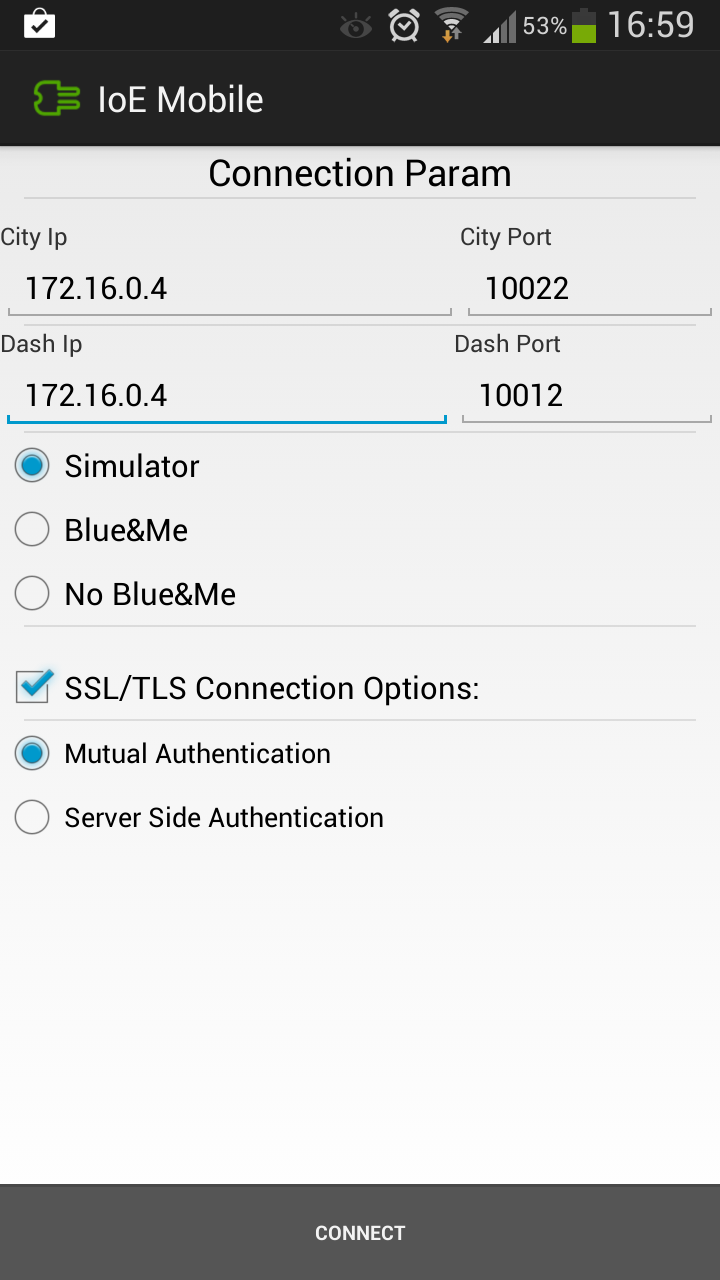
\includegraphics[width=\textwidth]{assets/mobile-app-main.png}
		\caption{Schermata Principale}
		\label{fig:main-activity}
	\end{subfigure}
	\begin{subfigure}{0.45\textwidth}
		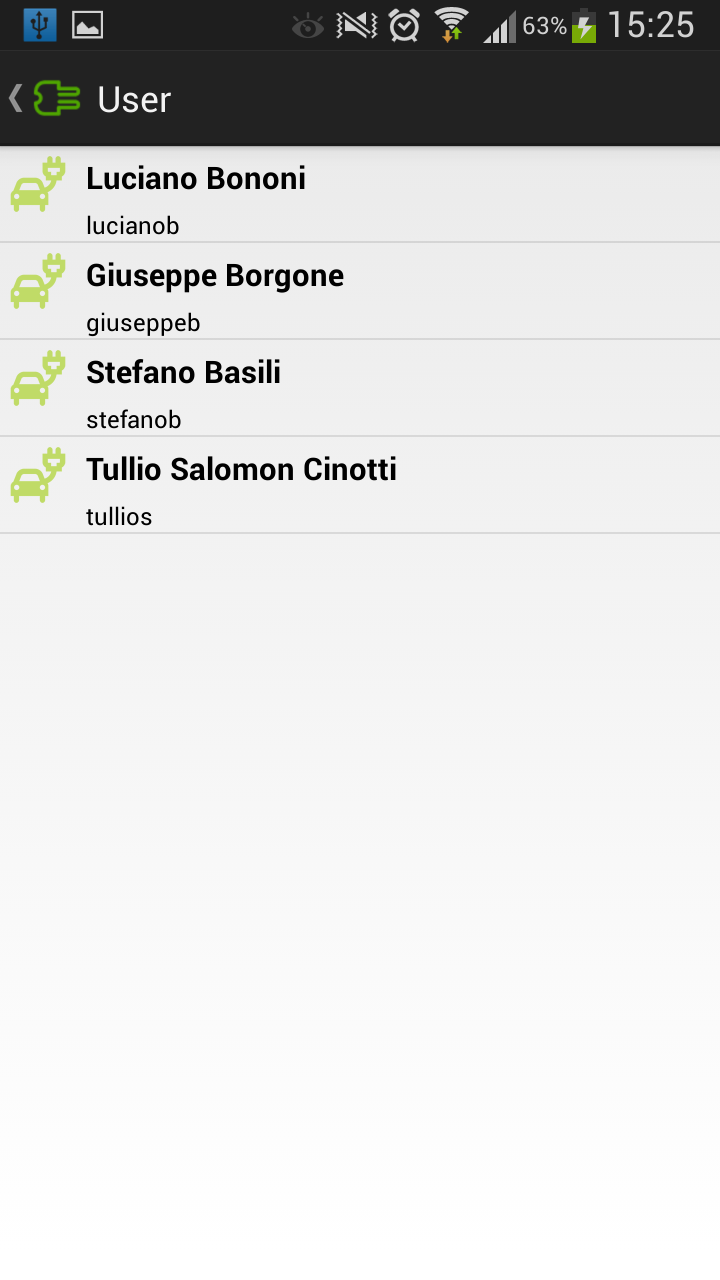
\includegraphics[width=\textwidth]{assets/mobile-app-select-user.png}
		\caption{Selezione Utente}
		\label{fig:select-user}
    \end{subfigure}
    	\begin{subfigure}{0.45\textwidth}
		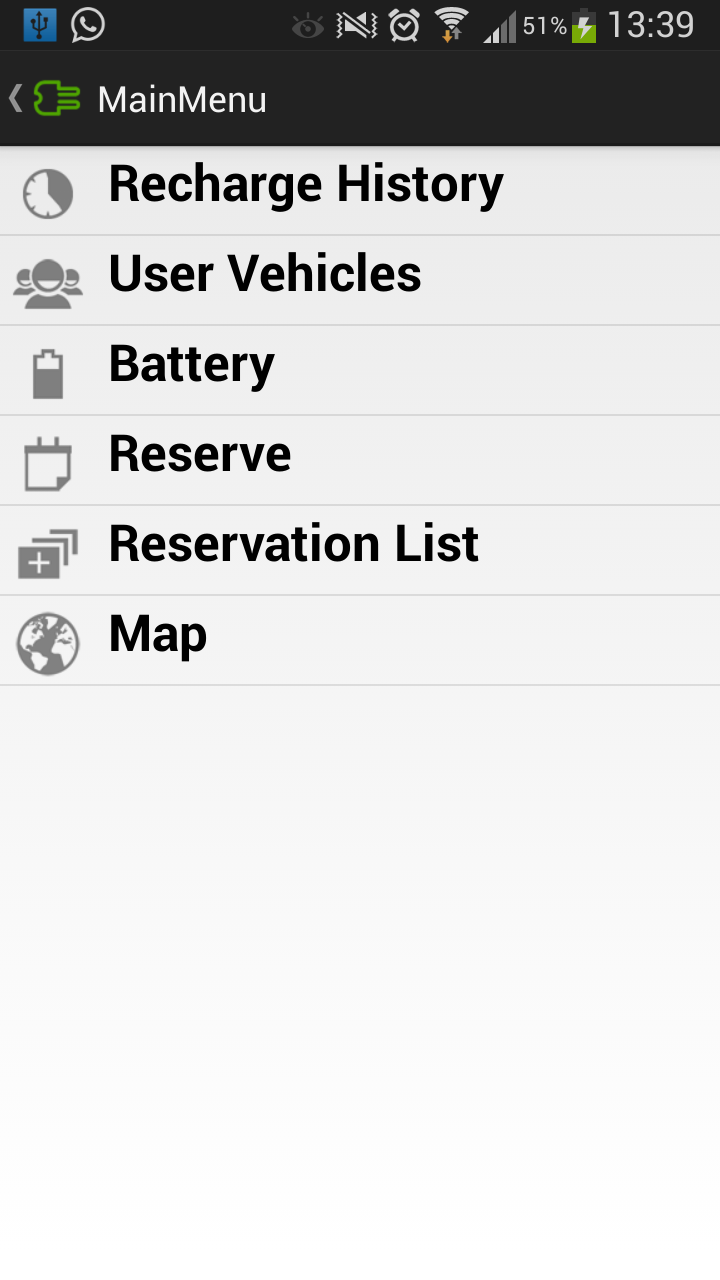
\includegraphics[width=\textwidth]{assets/mobile-app-main-menu.png}
		\caption{Menu Principale}
		\label{fig:main-menu}
	\end{subfigure}
	\begin{subfigure}{0.45\textwidth}
		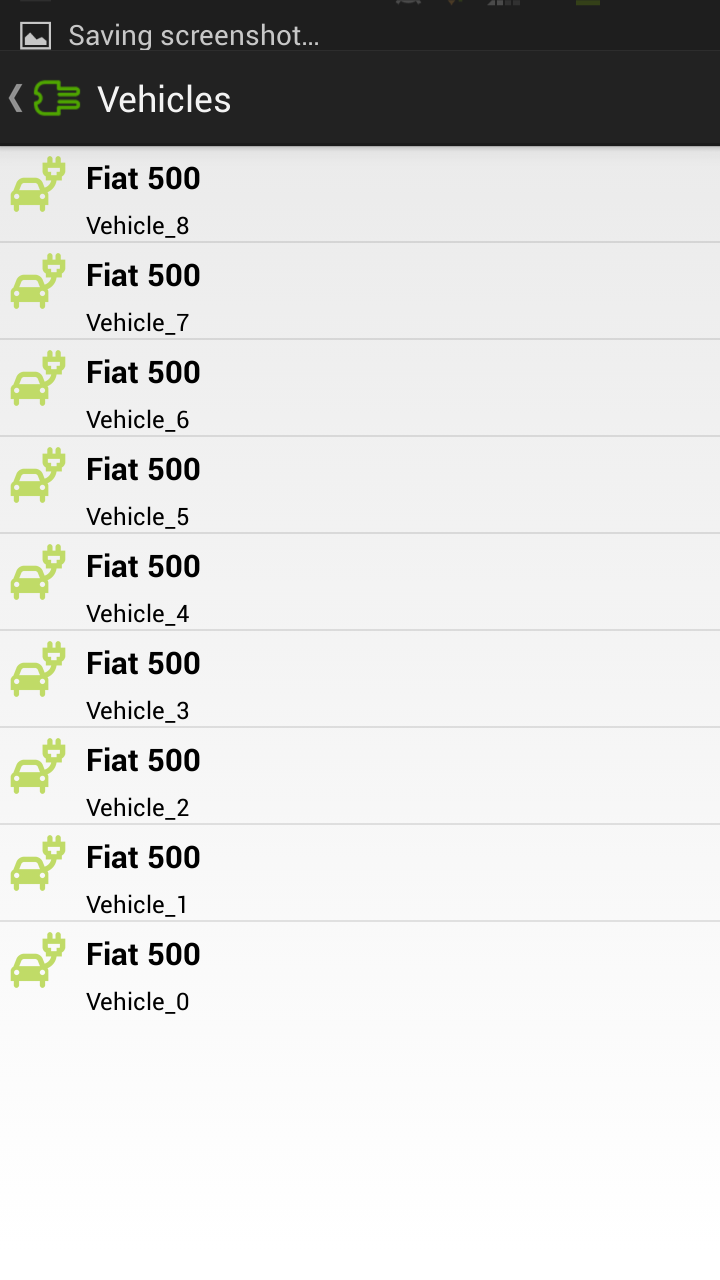
\includegraphics[width=\textwidth]{assets/mobile-app-select-veh.png}
		\caption{Selezione Veicolo}
		\label{fig:select-veh}
    \end{subfigure}
\end{figure}

\subsection{Simulazione}

Questa modalità permette di assumere il controllo di un veicolo contenuto nel simulatore. Questo deve essere avviato specificando un parametro che genera la scrittura dei dati relativi ai veicoli sul \emph{Dash SIB}. Ciò implica che, premuto il pulsante \emph{Connect}, (Fig. \ref{fig:main-activity}), bisogna selezionare ``Luciano Bononi'' ovvero l'utente di default usato dai veicoli del simulatore (Fig. \ref{fig:select-user}). Da questo momento l'applicazione non diverge molto dalla modalità di esecuzione con Blue\&{}Me salvo il fatto che le azioni intraprese avranno ripercussioni sul simulatore e non sul mondo reale.

\subsection{Con Blue\&{}Me}

Questa modalità viene usata in un contesto reale e richiede la presenza di un veicolo equipaggiato la tecnologia Blue\&{}Me di Fiat. Le informazioni relative alla batteria vengono prelevate tramite Bluetooth e scritte nel \emph{Dash SIB} per i motivi di interoperabilità spiegati nella Sez. \ref{subsec:dash-sib}. Le informazioni relative al GPS, non fornite dal veicolo, vengono prelevate dal GPS (o altre fonti) fornito dallo smartphone.

\subsection{Senza Blue\&{}Me}\label{subsec:noblueme}

Questa modalità d'uso è rivolta principalmente a chi vuole svolgere le attività di interazione con il CS senza essere a bordo del proprio veicolo. Questo comporta l'assenza della \emph{Dash SIB}: se invocata viene infatti inibita la scelta dei suoi parametri con conseguente inibizione del monitoraggio dei parametri del veicolo e relativa disabilitazione nel menu principale. Anche se la \emph{Dash SIB} fosse situata sul cellulare anziché sul veicolo risulterebbe comunque inservibile poiché il veicolo risulterebbe fuori portata o spento. Si possono comunque svolgere le operazioni di prenotazione e ritiro delle ricariche mantenendo monitorato lo stato di quelle già effettuate nonché la disponibilità di consultazione della mappa indicante le colonnine.

\section{Funzionalità}

In questa sezione eseguirò un analisi dettagliata delle funzionalità dell'applicazione. La descrizione cercherà di essere il più possibile funzionalità-centrica e non activity-centrica anche se spesso i due aspetti coincidono. 

\subsection{Il menu principale}

La prima schermata dell'applicazione consente permette di scegliere i parametri di connessione ai SIB (Fig. \ref{fig:main-activity}) e la modalità di esecuzione. Una volta premuto il tasto \emph{connect} si dovrà selezionare l'utente (Fig. \ref{fig:select-user}) per accedere al menu principale (Fig. \ref{fig:main-menu}).

Questo apparirà con due cole opzioni, \emph{Recharge History} e \emph{Select Vehicle}, poiché tutte le altre opzioni dipendono dal veicolo che si sta utilizzando e quindi non vengono mostrate finché non se ne sceglie uno mediante l'apposito menu (Fig. \ref{fig:select-veh}). 

\subsection{Storia delle ricariche effettuate}

In questa schermata (Fig. \ref{fig:recharge-history}) possiamo monitorare la storia delle ricariche effettuate. Questa parte è stata introdotta anche per dimostrare l'interoperabilità del nostro sistema con uno SIB-based sviluppato dalla spagnola AICIA.

\subsection{Monitoraggio Parametri Batteria}

Dal menu principale si può accedere al monitoraggio dei parametri della batteria attraverso l'opzione \emph{Battery}. Vengono visualizzati sia i parametri variabili (Fig. \ref{fig:battery-var}) che quelli nominali (Fig. \ref{fig:battery-nom}). I dati relativi all'intensità di corrente e al voltaggio sono visibili solo se si è connessi a un veicolo reale tramite Blue\&{}Me in quanto il nostro modello di simulazione non li implementa. I dati nominali sono disponibili nella modalità di simulazione ma non in quella reale poiché queste informazioni non vengono fornite dalla centralina del veicolo.

\begin{figure}
	\centering
	\begin{subfigure}{0.45\textwidth}
		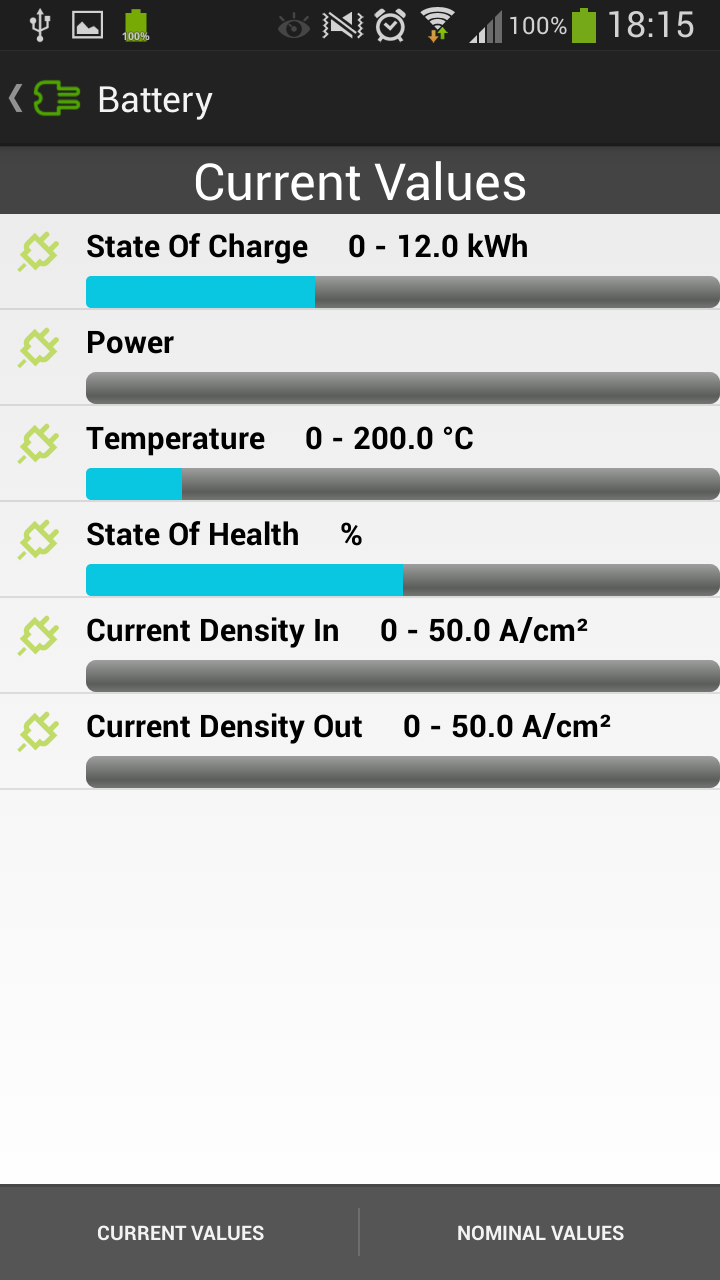
\includegraphics[width=\textwidth]{assets/mobile-app-battery-var.png}
		\caption{Dati variabili della batteria}
		\label{fig:battery-var}
	\end{subfigure}
	\begin{subfigure}{0.45\textwidth}
		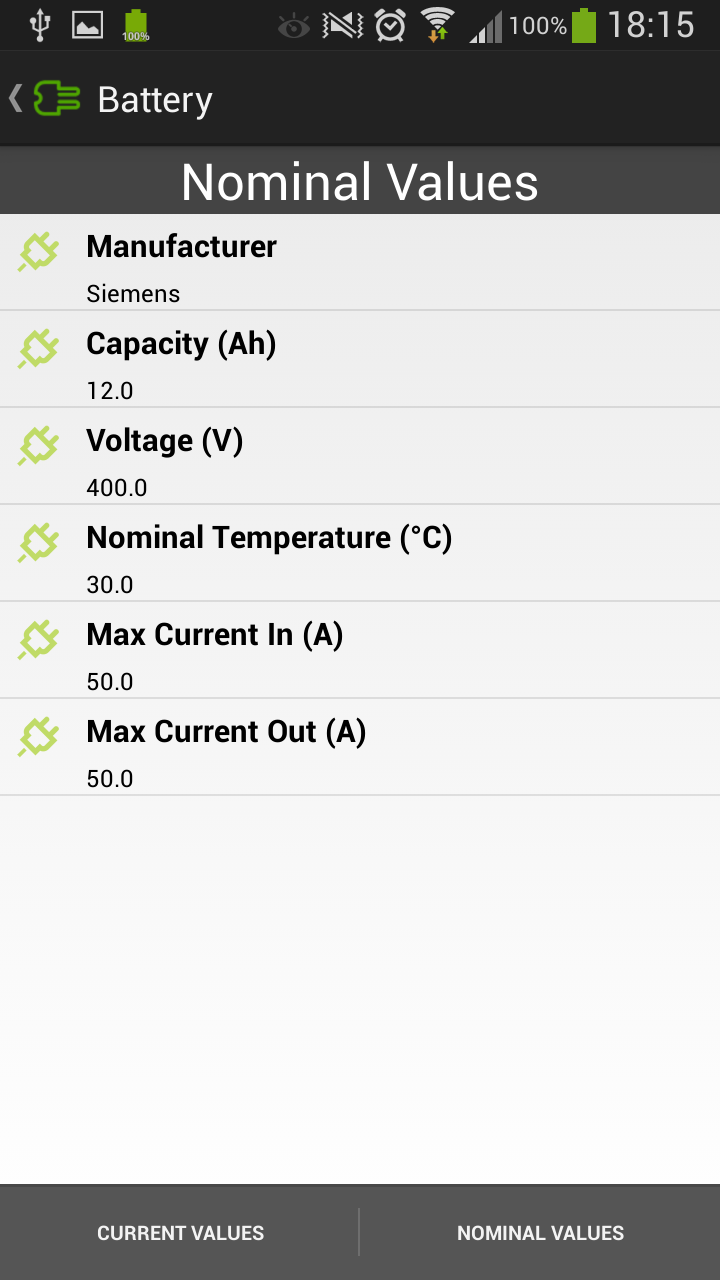
\includegraphics[width=\textwidth]{assets/mobile-app-battery-nom.png}
		\caption{Dati fissi della batteria}
		\label{fig:battery-nom}
    \end{subfigure}
    \begin{subfigure}{0.45\textwidth}
		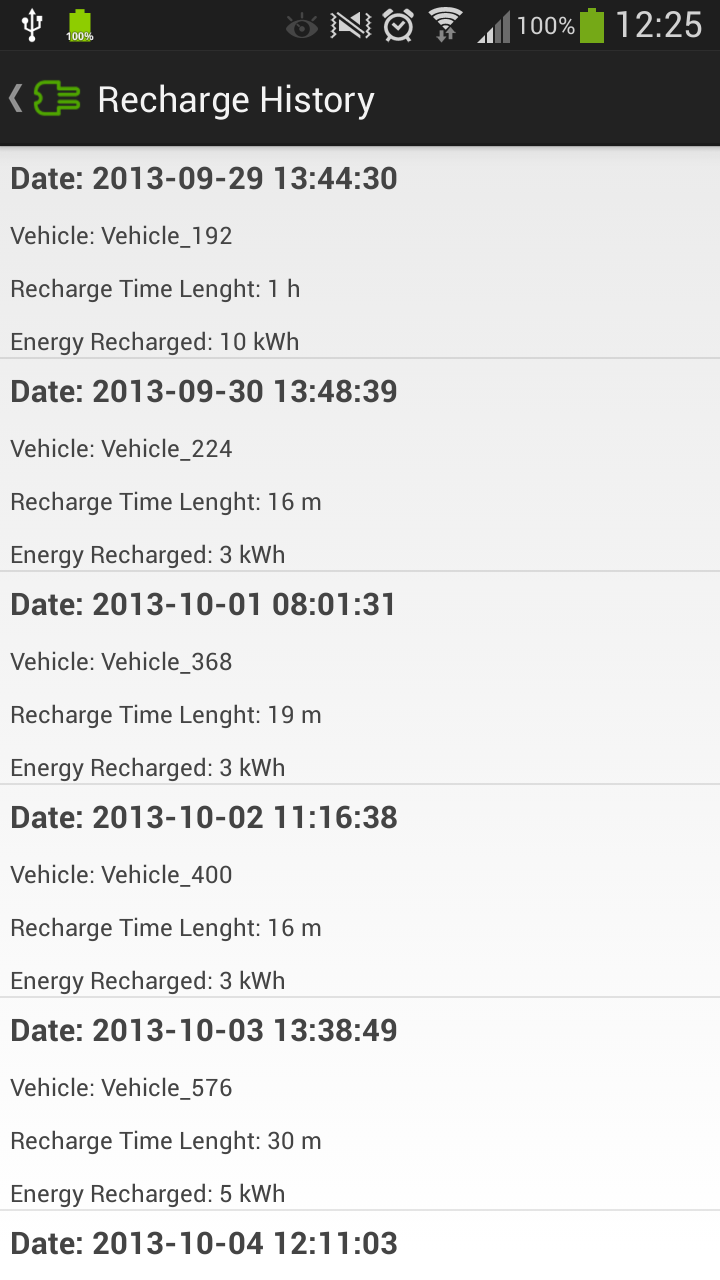
\includegraphics[width=\textwidth]{assets/mobile-app-recharge-history.png}
		\caption{Storia Ricariche}
		\label{fig:recharge-history}
	\end{subfigure}
	\begin{subfigure}{0.45\textwidth}
		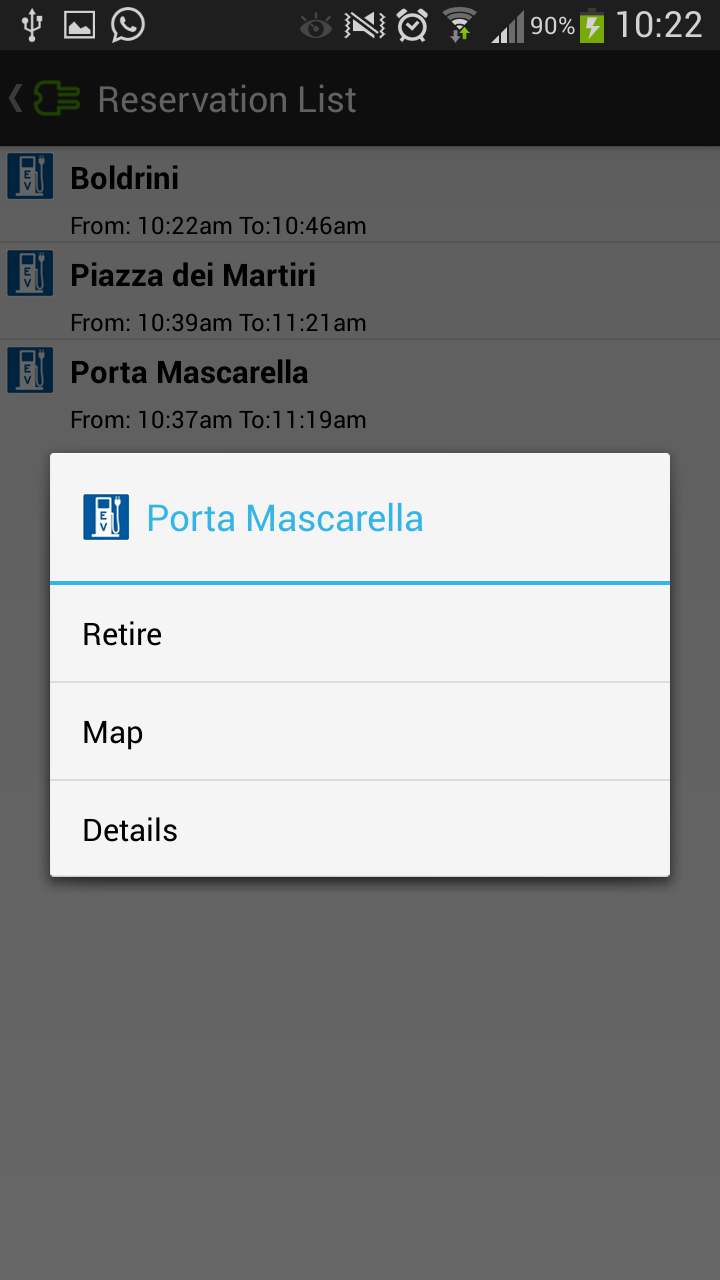
\includegraphics[width=\textwidth]{assets/mobile-app-reservation.png}
		\caption{Selezione Veicolo}
		\label{fig:reservation}
    \end{subfigure}
\end{figure}

\subsection{Effettuare una richiesta di prenotazione}

Per accedere a questa funzionalità si seleziona \emph{Reserve} dal menu principale. Appare la schermata che consente di impostare i parametri necessari per inoltrare una richiesta di prenotazione al CS. Come si può vedere in figura \ref{fig:charge-request} il servizio rende disponibili diverse opzioni per personalizzare il processo di prenotazione. Essenzialmente la schermata consente di dare una veste grafica al protocollo di richiesta descritto nella sezione \ref{sec:protocol}.

\subsubsection{Creazione della richiesta}

La scelta dell'area entro la quale verificare la disponibilità di colonnine assume di default la posizione del veicolo come punto centrale. Se questa non è disponibile (modalità \emph{Senza Blue\&{}Me}, Sez. \ref{subsec:noblueme}) l'utente è costretto a selezionarne una dalla mappa. Per accedere alla funzione di selezione del punto si clicca sul pulsante \emph{Map} che mostra la mappa centrata sulla città in cui ci si trova e tramite un tocco sullo schermo si sceglie il punto di interesse (Fig \ref{fig:map-chooser}).

Selezionata l'area di interesse si procede alla selezione del raggio di ricerca impostato di default è impostato a 6 km con un massimo di 15 km: oltre non avrebbe senso in quanto sarebbe più idoneo spostare il punto di interesse.

La barra di selezione della quantità di energia ha come dimensione massima la capacità della batteria. L'immagine in Fig. \ref{fig:charge-request} è relativa a una batteria con capacità 40 kWh e una quantità di energia residua di 12 kWh indicato dal colore rosso dei numeri a destra della barra. Lo spostamento del cursore verso destra è proporzionale alla quantità di energia che si intende acquistare: conseguentemente il numero a destra indica gradualmente la quantità che dovrà avere la batteria al termine della carica rapportata a quella massima raggiungibile: l'effettiva quantità di carica richiesta sarà determinata dalla differenza tra il valore selezionato e la quantità di carica iniziale. A questo punto il cursore assume colore nero indicando che si può procedere con la richiesta. Il procedimento è inibito finché non si acquista almeno 1 kWh. 

Nel caso in cui la capacità della batteria e la quantità di carica non siano disponibili (modalità \emph{Senza Blue\&{}Me}) viene data la possibilità di scegliere qualunque quantità di energia e l'utente viene allertato dell'eventualità di poter acquistare più energia di quella quella massima supportabile dalla batteria del veicolo.

L'ultimo parametro da impostare è l'intervallo di tempo massimo entro il quale l'utente eseguire la ricarica con un lasso temporale di default di 3 ore variabile grazie agli appositi pulsanti di selezione di data/ora con relativi controlli di congruenza.

A questo l'apposito pulsante in alto a destra consente l'invio della richiesta.

\subsubsection{Scelta della risposta}

In seguito all'invio della richiesta viene mostrato all'utente un messaggio che invita ad attendere la risposta. In caso di fallimento della richiesta l'utente viene allertato e rimandato nella schermata di richiesta con l'invito di cambiare i parametri. In caso di successo appare una schermata con le opzioni di ricarica restituite dal servizio cittadino. La Fig. \ref{fig:charge-options} indica le relative informazioni:

\begin{itemize}
	\item Nome del GCP presso cui avverrà la ricarica.
	\item Distanza reale dal GCP calcolata grazie alla libreria UniboGeoTools.
	\item Orario e prezzo della ricarica.
	\item Energia stimata per raggiungere la colonnina.
	\item Dislivello in salita e in discesa.
\end{itemize}

Le informazioni sul profilo altimetrico ed il contributo energetico vengono mostrate in una schermata a parte accessibile tramite un apposito menu visualizzabile tenendo premuta a lungo un opzione di ricarica (Fig. \ref{fig:charge-options-menu}), aspetto approfondito nella sezione (\ref{subsec:altimetry}).

Viene data inoltre la possibilità di eseguire operazioni di ordinamento delle varie ricariche in base ai parametri sopra elencati ovvero: distanza, prezzo, orario, contributo energetico ecc.. Infine, volendo, si possono visualizzare le opzioni di ricarica sulla mappa. Premendo su una di esse viene disegnato il percorso fino alla relativa colonnina. I tratti in salita sono colorati di rosso, quelli in discesa di verde e quelli in pianura di grigio. Le caratteristiche della mappa sono comunque approfondite nella Sez. \ref{subsec:map}.

Scegliendo l'opzione di ricarica viene eseguita la parte restante del protocollo e nel caso in cui sia ancora valida allora verrà mostrata la schermata indicante le prenotazioni attive per l'utente (Fig. \ref{fig:reservation}).

\subsection{Visualizzazione e Ritiro delle Prenotazioni}

In questa schermata vengono visualizzate le prenotazioni pendenti per l'utente (Fig. \ref{fig:reservation}). È accessibile tramite il menu principale \emph{Reservation List} o raggiunta automaticamente se viene confermata dal sistema l'opzione di ricarica selezionata durante il processo di prenotazione. 

Selezionando una prenotazione apparirà un menu che permette di mostrarla sulla mappa oppure di ritirarla.

\begin{figure}
	\centering
	\begin{subfigure}{0.45\textwidth}
		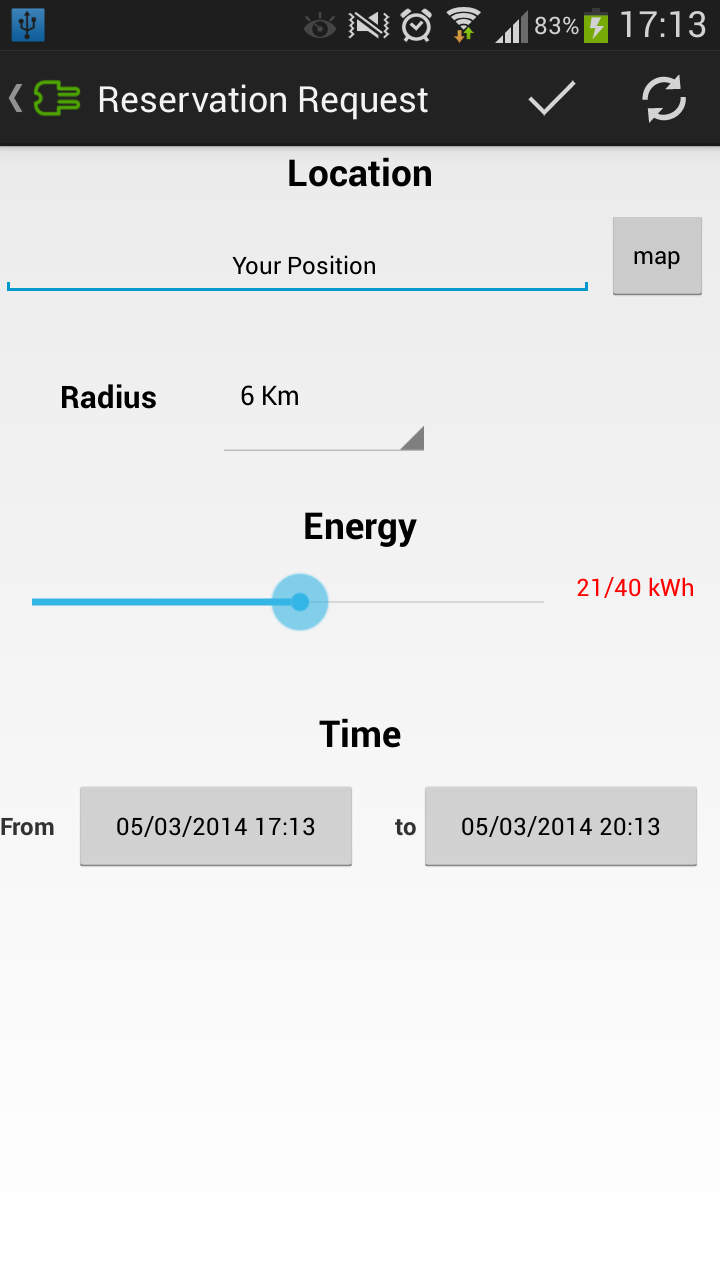
\includegraphics[width=\textwidth]{assets/mobile-app-charge-request.png}
		\caption{Inserimento Prenotazione}
		\label{fig:charge-request}
	\end{subfigure}
	\begin{subfigure}{0.45\textwidth}
		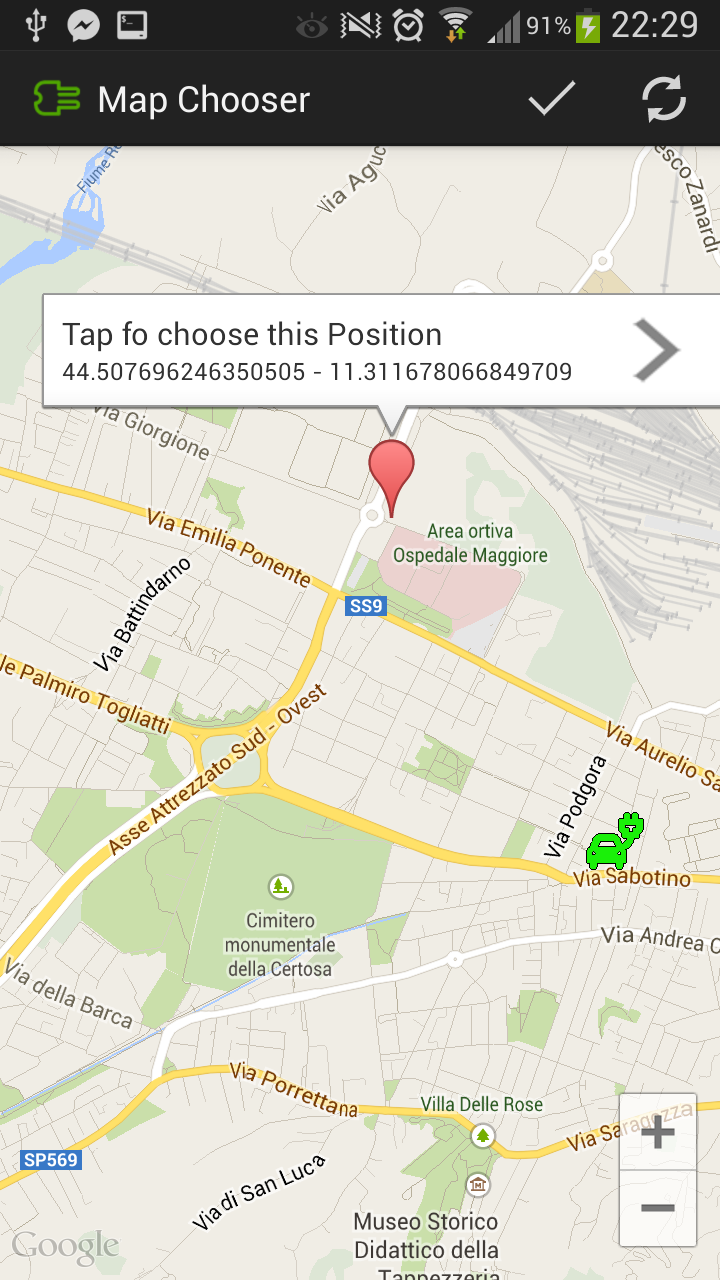
\includegraphics[width=\textwidth]{assets/mobile-app-map-chooser.png}
		\caption{Scelta di un punto nella mappa}
		\label{fig:map-chooser}
	\end{subfigure}
	\begin{subfigure}{0.45\textwidth}
		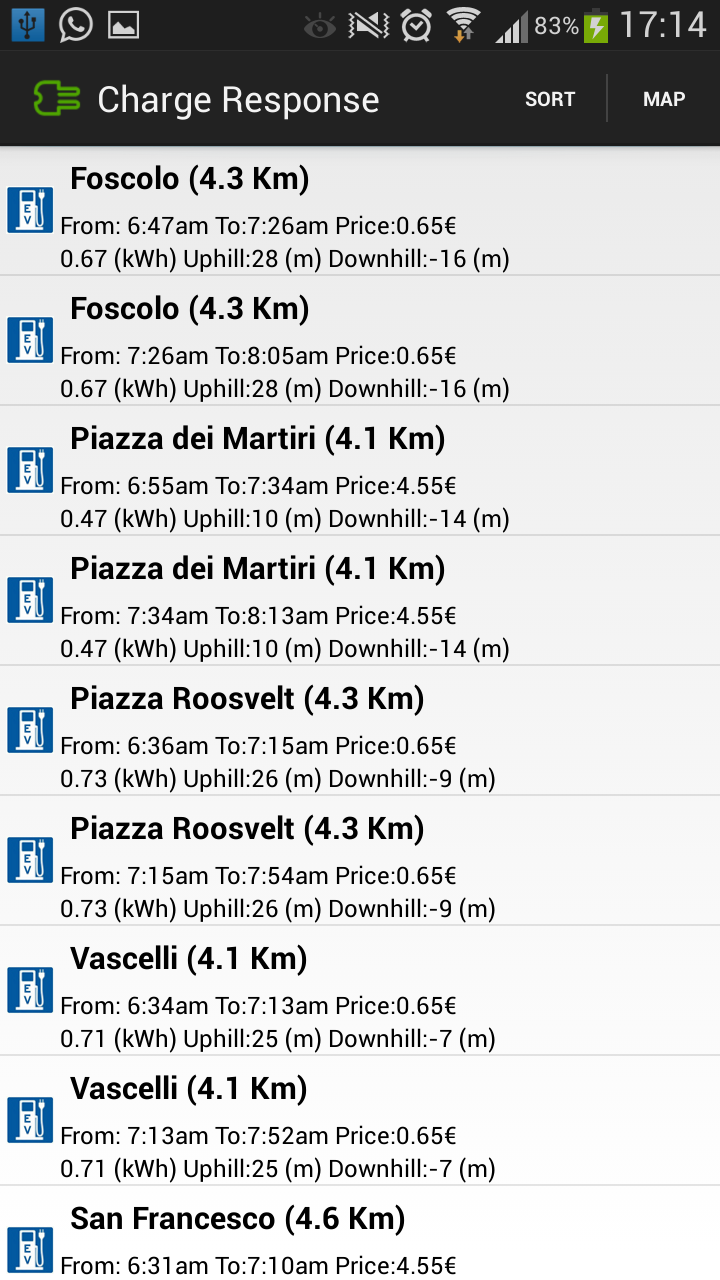
\includegraphics[width=\textwidth]{assets/mobile-app-charge-options.png}
		\caption{Visualizzazione opzioni di ricarica}
		\label{fig:charge-options}
    \end{subfigure}
	\begin{subfigure}{0.45\textwidth}
		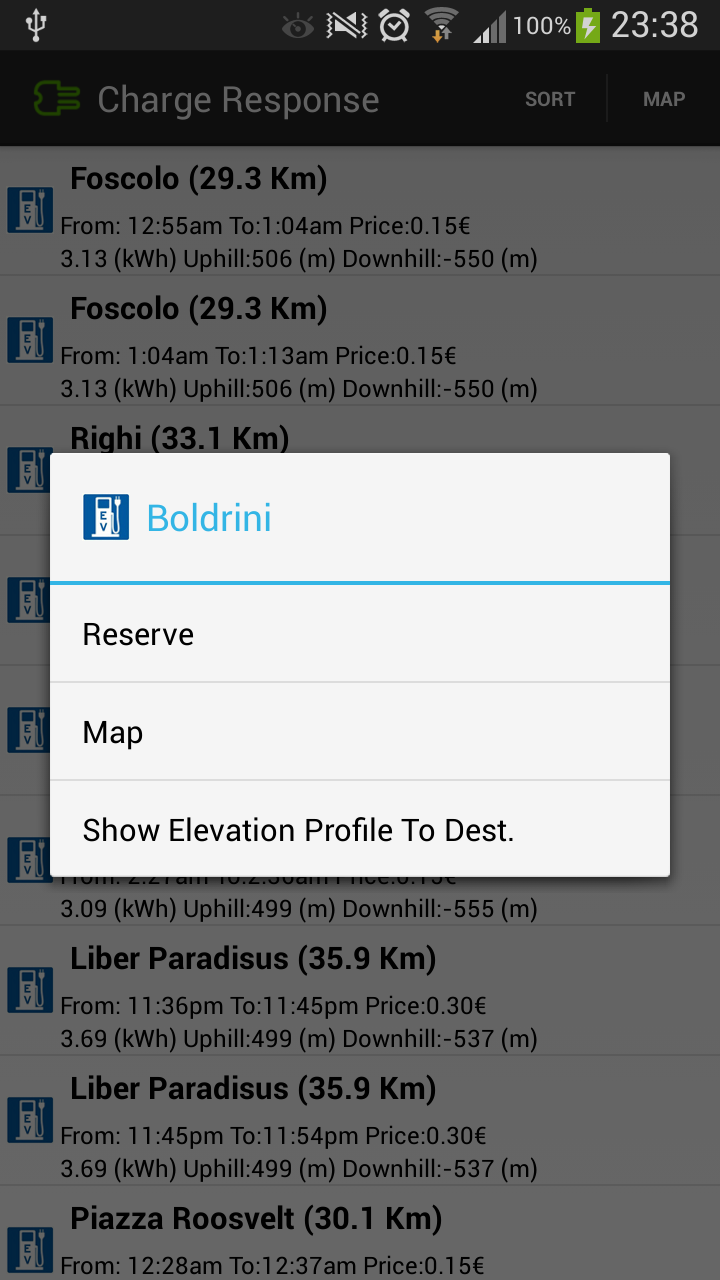
\includegraphics[width=\textwidth]{assets/mobile-app-charge-options-menu.png}
		\caption{Menu opzioni di ricarica}
		\label{fig:charge-options-menu}
    \end{subfigure}
\end{figure}

\subsection{Profilo Altimetrico e Consumo Energetico}\label{subsec:altimetry}

Il profilo altimetrico è una delle feature più innovative introdotte nell'applicazione. Può rivelarsi di fondamentale importanza per l'utente che, grazie ad essa, può scegliere il percorso migliore per raggiungere la sua destinazione. Come vedremo nella sezione relativa al modello della batteria (\ref{sec:battery}), i veicoli elettrici possono recuperare energia grazie alla frenata rigenerativa e allo sfruttamento delle discese. Strade con molti tratti in discesa possono portare a un recupero di energia non indifferente. 

La libreria UniboGeoTools, usata a questo scopo, permette inoltre di eseguire stime dell'energia necessaria a percorre un determinato tratto di strada. Queste informazioni sono mostrate nella schermata \emph{Elevation Profile}:

\begin{itemize}
	\item \textbf{Path Altimetry Summary}: informazioni riassuntive sul viaggio che l'utente sta per intraprendere. Come mostrato in Fig. \ref{fig:altimetry-1}, oltre alle informazioni di destinazione, distanza e peso viene fornita una stima sull'energia totale che impiegherà il veicolo per raggiungere la destinazione oltre alle informazioni su quanta discesa, salita e pianura caratterizzano il percorso.
	\item \textbf{Cumulative Altimetry Offset}: il riquadro fornisce informazioni sul dislivello che caratterizza il percorso (Fig \ref{fig:altimetry-1}).
	\item \textbf{Average Slope}: fornisce informazioni sulla pendenza media che caratterizza il percorso. Importante in quanto, come detto prima, una pendenza significativa può portare ad elevati consumi oppure a un ricavo di energia (Fig \ref{fig:altimetry-1}).
	\item \textbf{Max Slope}: fornisce informazioni di massima sulla pendenza del percorso, ovvero la pendenza massima che troveremo in salita e in discesa (Fig \ref{fig:altimetry-2}).
	\item \textbf{Elevation Dependent Energy Ref}: informazioni sul contributo energetico necessario per vincere il dislivello. A tal scopo viene utilizzata l'energia potenziale gravitazionale (Fig \ref{fig:altimetry-2}).
	\item \textbf{Energy Profile for Path Lenght}: energia impiegata per percorrere il tragitto. Nel caso precedente veniva preso in considerazione unicamente il dislivello; qui viene invece considerata anche la distanza che separa l'utente dalla destinazione (Fig \ref{fig:altimetry-2}).
	\item \textbf{Altitude Graph}: grafico che mostra il profilo altimetrico che ci separa dalla destinazione. Sono indicati in verde i tratti in discesa e in rosso quelli in salita (Fig \ref{fig:altimetry-3}).
\end{itemize} 
\noindent
Ulteriori informazioni sul profilo altimetrico vengono fornite sulla mappa, come approfondito nella Sez. \ref{subsec:map}.

\begin{figure}
	\centering
	\begin{subfigure}{0.45\textwidth}
		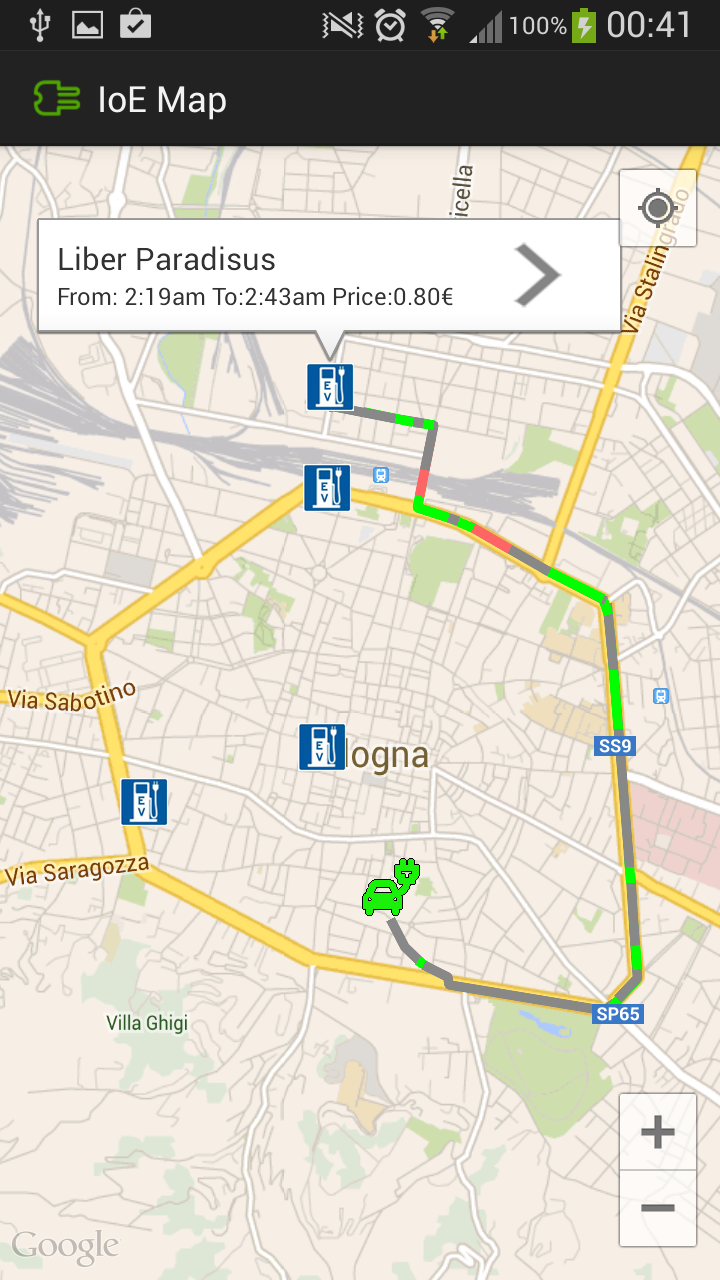
\includegraphics[width=\textwidth]{assets/mobile-app-map.png}
		\caption{Mappa con Profilo Altimetrico}
		\label{fig:map-altimetry}
	\end{subfigure}
	\begin{subfigure}{0.45\textwidth}
		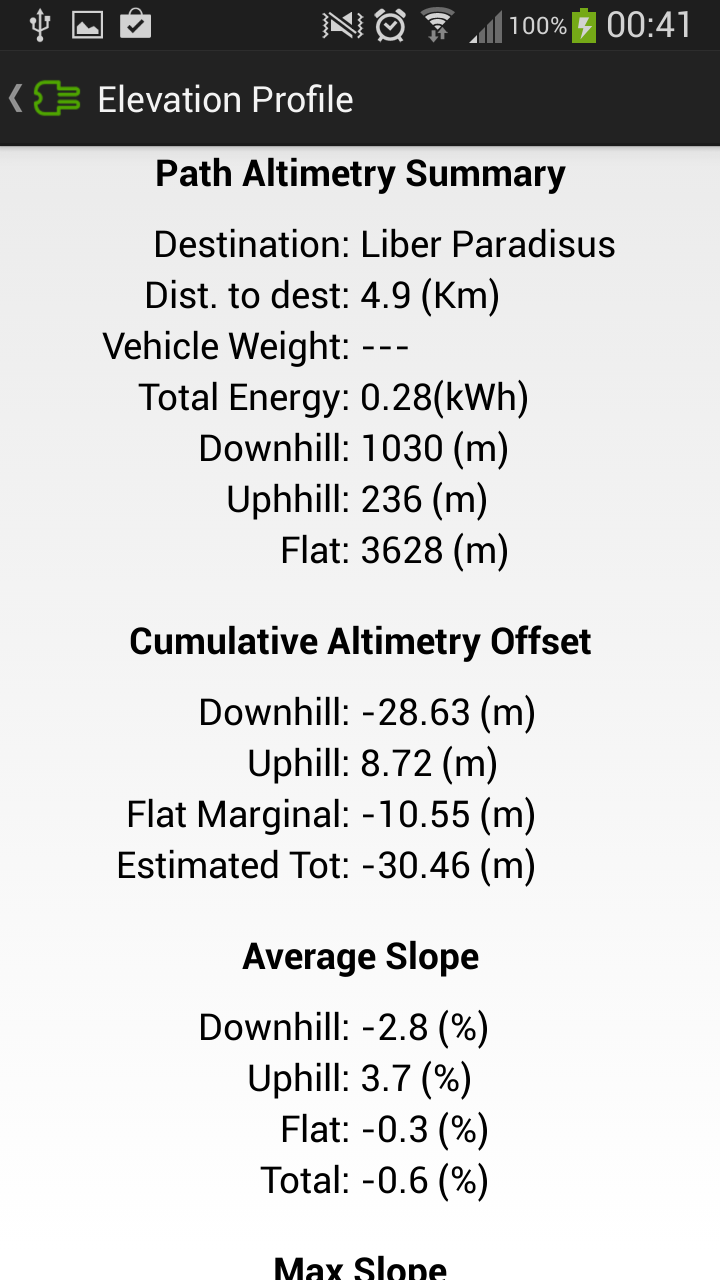
\includegraphics[width=\textwidth]{assets/mobile-app-altimetry-1.png}
		\caption{Scelta di un punto nella mappa}
		\label{fig:altimetry-1}
	\end{subfigure}
	\begin{subfigure}{0.45\textwidth}
		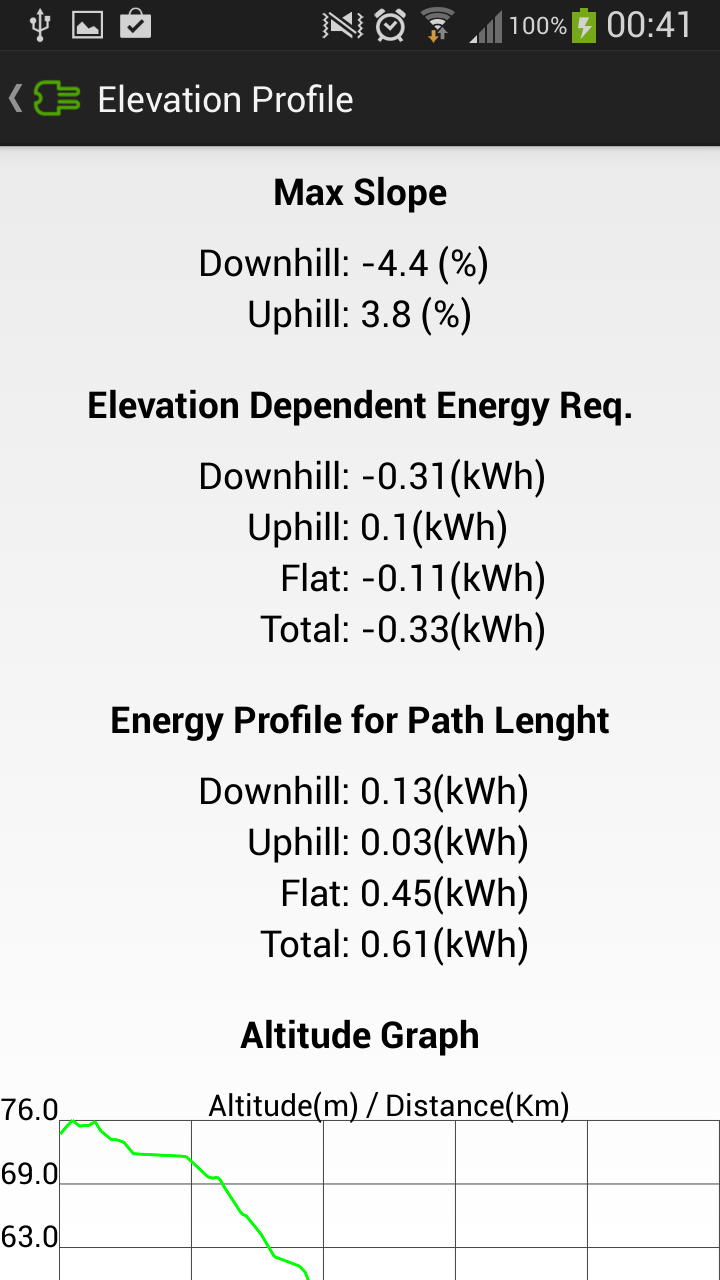
\includegraphics[width=\textwidth]{assets/mobile-app-altimetry-2.png}
		\caption{Visualizzazione opzioni di ricarica}
		\label{fig:altimetry-2}
    \end{subfigure}
	\begin{subfigure}{0.45\textwidth}
		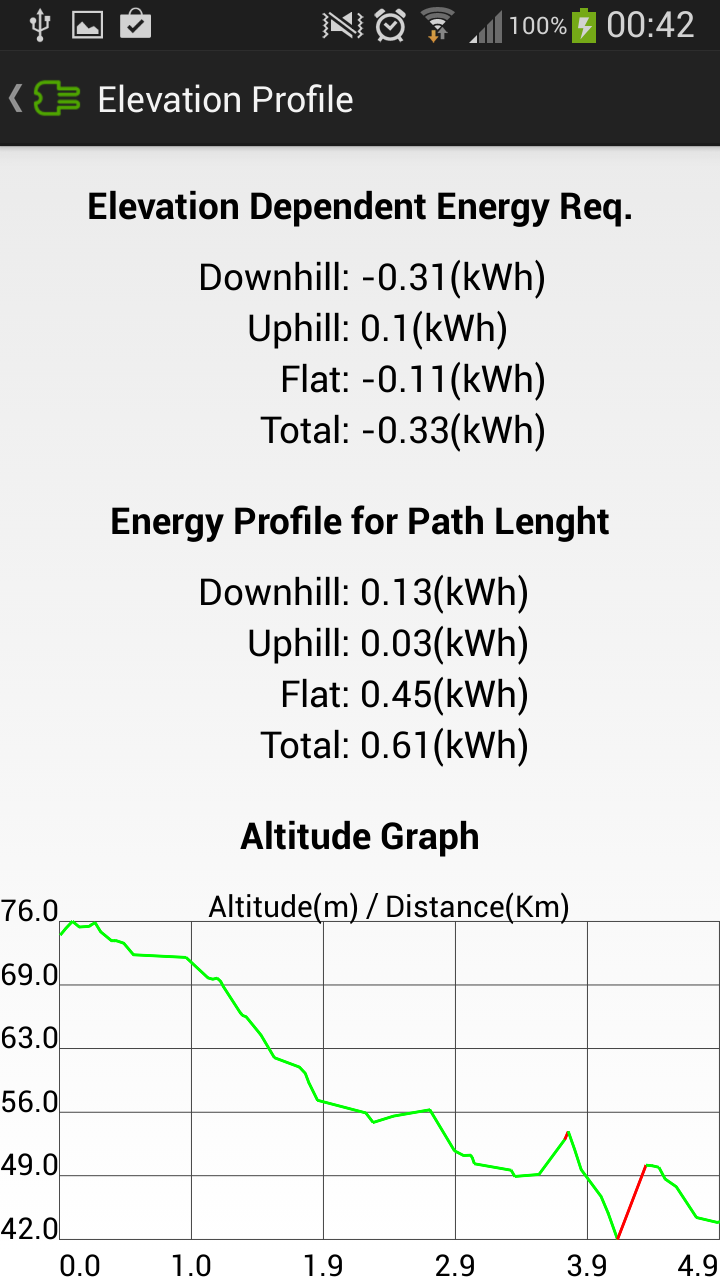
\includegraphics[width=\textwidth]{assets/mobile-app-altimetry-3.png}
		\caption{Menu opzioni di ricarica}
		\label{fig:altimetry-3}
    \end{subfigure}
\end{figure}

\subsection{Mappa}\label{subsec:map}

La mappa viene centrata sulla città di riferimento. Su di essa si può vedere il veicolo in movimento, sia simulato che reale. Premendo il pulsante di localizzazione in alto a destra si effettuato lo zoom sul veicolo. Alla mappa si può accedere in diverse occasioni:

\begin{itemize}
	\item \textbf{Dal menu principale}: selezionando \emph{Map} si accede alla mappa che mostrerà i GCP della città con possibilità di effettuare una prenotazione cliccando su quello di interesse (Fig. \ref{fig:map-gcp}).
	\item \textbf{Scelta delle Opzioni Ricarica}: le opzioni di carica restituite dal CS possono essere visualizzate sulla mappa. Se scegliamo di visualizzare la mappa a partire da un opzione di ricarica, verrà anche disegnato il percorso che ci separa dalla colonnina. Viceversa verranno visualizzate tutte le colonnine e per evidenziare il percorso si dovrà selezionare quella di interesse (Fig. \ref{fig:map-altimetry}). 
	\item \textbf{Prenotazioni}: dalla schermata delle prenotazioni pendenti possiamo visualizzarle sulla mappa con possibilità di effettuare il ritiro dell'operazione di ritiro semplicemente selezionando la colonnina associata.
\end{itemize}

Come mostrato in Fig. \ref{fig:map-altimetry} viene disegnato il percorso che ci separa dalla destinazione evidenziando in verde i tratti in discesa, in rosso quelli in salita e in grigio quelli.

Premendo su una delle colonnine visualizzate nella mappa viene aperto un popup che mostra informazioni sommarie sul GCP. Una freccia che permette di accedere a un menu con altre opzioni (Fig. \ref{fig:map-menu}). Dal quale si può eseguire una prenotazione, consultare i dettagli sul profilo altimetrico o aprire il navigatore reso disponibile dal Sistema Operativo usando come punto di partenza quello dove ci si trova e come punto di destinazione quello selezionato sulla mappa (Fig. \ref{fig:navigator}).

\section{Notifica batteria Scarica}

Quando la carica della batteria scende al di sotto di una certa soglia, attualmente impostata al 30\% della carica nominale, viene inviata all'utente una notifica che appare nell'omonima area resa disponibile dai Sistemi Operativi Android (Fig. \ref{fig:notify}). La notifica viene reiterata a salti di 5\% di scarica della batteria. Premendo sulla notifica si apre la schermata destinata alle prenotazioni.

\begin{figure}
	\centering
	\begin{subfigure}{0.45\textwidth}
		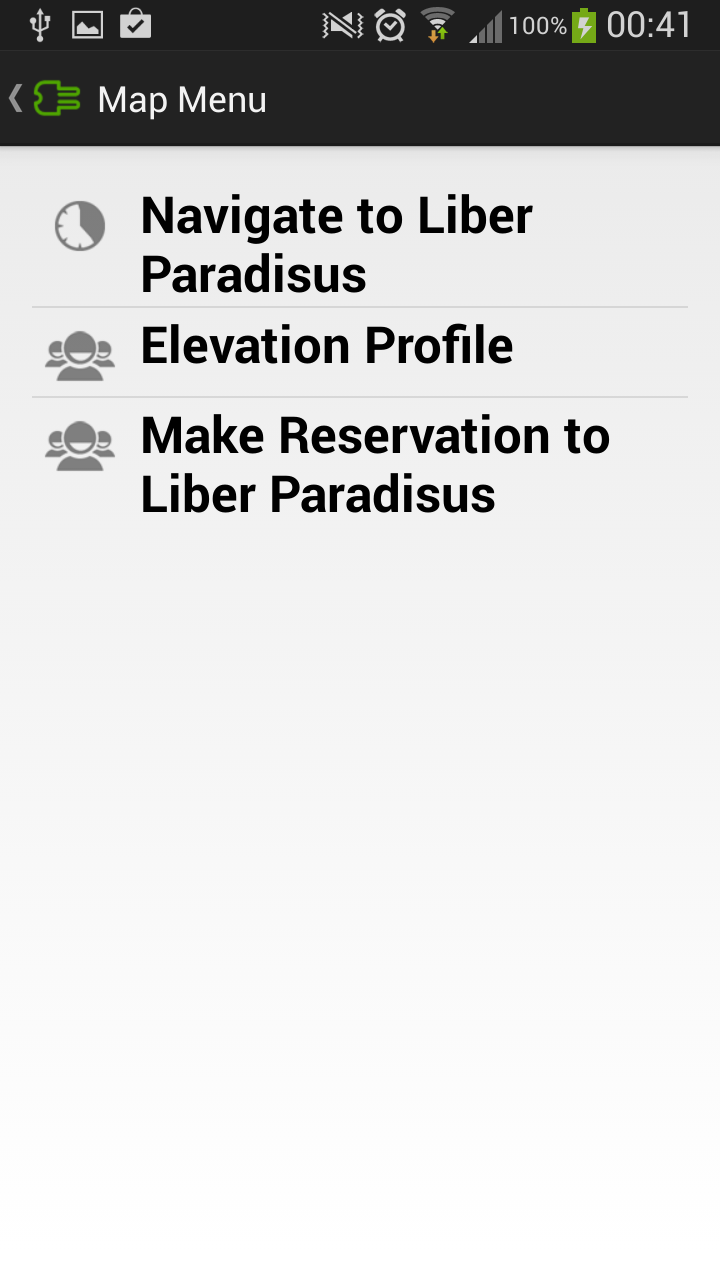
\includegraphics[width=\textwidth]{assets/mobile-app-map-menu.png}
		\caption{Menu Mappa}
		\label{fig:map-menu}
	\end{subfigure}
	\begin{subfigure}{0.45\textwidth}
		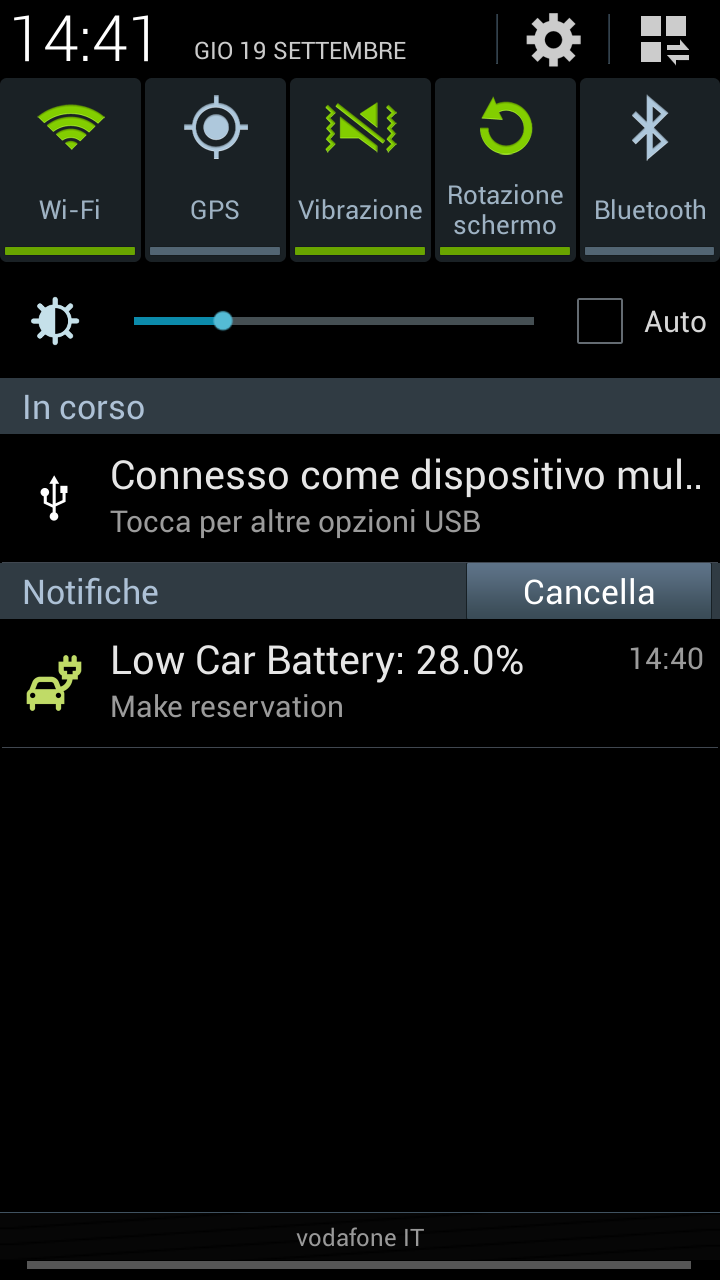
\includegraphics[width=\textwidth]{assets/mobile-app-notify.png}
		\caption{Notifica batteria scarica}
		\label{fig:notify}
	\end{subfigure}
	\begin{subfigure}{0.45\textwidth}
		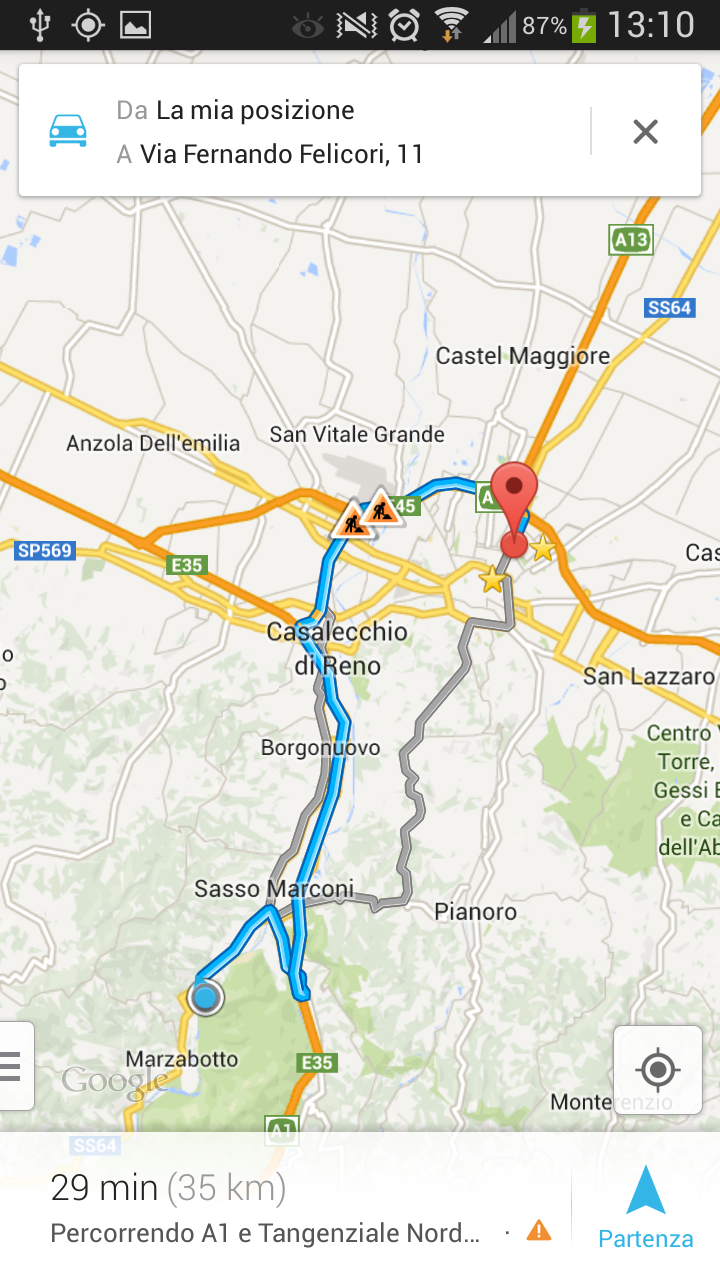
\includegraphics[width=\textwidth]{assets/mobile-app-navigator.png}
		\caption{Navigatore Satellitare}
		\label{fig:navigator}
    \end{subfigure}
	\begin{subfigure}{0.45\textwidth}
		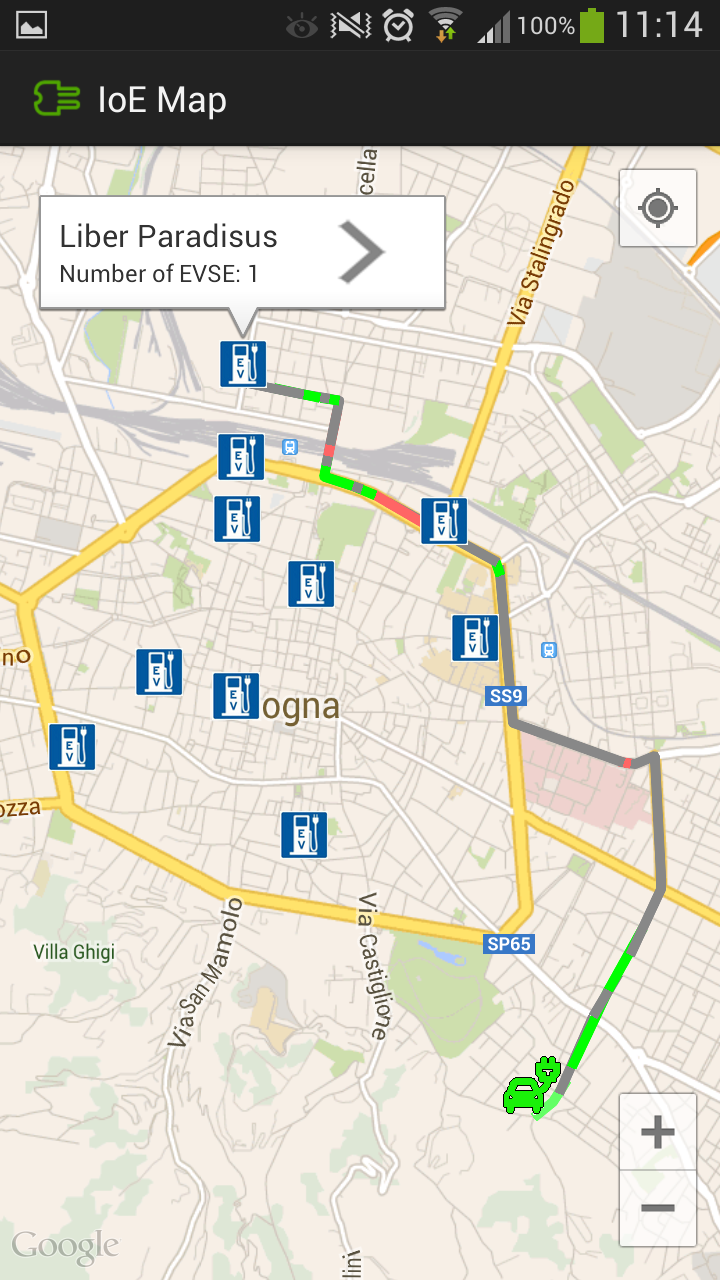
\includegraphics[width=\textwidth]{assets/mobile-app-map-gcp.png}
		\caption{Visione di tutti i GCP della città}
		\label{fig:map-gcp}
    \end{subfigure}
\end{figure}

\section{Implementazione}


\subsection{Implementazione}

\subsection{Operazioni Asincrone}

Tutte le operazioni che prevedono l'utilizzo della rete, quindi potenzialmente lunghe, sono eseguite all'interno di un \code{AsyncTask} ovvero una classe messa a disposizione dalla libreria di base di Android che permette di eseguire operazioni asincrone e contemporaneamente aggiornare l'interfaccia grafica. Questo da un lato permette di avere un applicazione fluida in quanto l'interfaccia non rimane bloccata in attesa dei risultati e dall'altro evita il verificarsi di errori dovuti al fatto che Android non permette di modificare l'interfaccia da un thread diverso da quello destinato al disegno di quest'ultima.

La maggior parte delle operazioni effettuate tramite rete, quindi nel nostro caso scambio di dati con i SIB, reperisce liste di elementi (veicoli, utenti, prenotazioni ecc..) che vengono mostrate all'interno di un apposita tipologia di Activity di Android le \code{ListActivity}.

Al fine di semplificare la programmazione delle Activity che contengono liste i quali elementi sono reperiti tramite la rete, ho creato la classe \code{ListLoaderTask<T>} che ne facilita il caricamento asincrono.

\subsection{Activities}

\subsection{Servizi}